\pdfoutput=1
\documentclass[12pt,a4paper]{article}
\usepackage[utf8]{inputenc}
\usepackage{amsmath}
\usepackage{amsfonts}
\usepackage{amssymb}
\usepackage{amsthm}
\usepackage[margin=0.7in]{geometry}
\usepackage{graphicx}
\usepackage{todonotes}
\usepackage{natbib}
\usepackage{url}
\usepackage[boxruled,vlined,linesnumbered]{algorithm2e}
\usepackage{caption}
\usepackage{subcaption}
\usepackage{lineno}
\usepackage{tcolorbox}
\usepackage{caption}
\usepackage{hyperref}
\usepackage{marginnote}
\AtBeginDocument{\let\textlabel\label}
\hypersetup{colorlinks=true,linkcolor=black,citecolor=black,filecolor=black,urlcolor=black}


\author{Jonathan Rosenblatt \\ Ben Gurion University}

%% OPTIONAL MACRO DEFINITIONS
\renewcommand*{\marginfont}{\scriptsize }

\newcommand{\reals}{\mathbb{R}} % the set of real numbers
\newcommand{\argmin}[2]{\textstyle{\mathop{argmin}_{#1}}\set{#2}} % The argmin operator
\newcommand{\argmax}[2]{\textstyle{\mathop{argmax}_{#1}}\set{#2}} % The argmin operator
\newcommand{\manifold}{\mathcal{M}} % A manifold.
\newcommand{\project}{\hookrightarrow} % The orthogonal projection operator.
\newcommand{\projectMat}{H} % A projection matrix.
\newcommand{\encode}{E} % a linear encoding matrix
\newcommand{\decode}{D} % a linear decoding matrix
\DeclareMathOperator{\Tr}{Tr}
\newcommand{\set}[1]{\{ #1 \}} % A set
\newcommand{\setII}[1]{\left\{ #1 \right\}} % A set
\newcommand{\rv}[1]{\mathbf{#1}} % A random variable
\newcommand{\x}{\rv x} % The random variable x 
\newcommand{\y}{\rv y} % The random variable x 
\newcommand{\U}{\rv u} % The random variable x 
\newcommand{\T}{\rv t} % The random variable x 
\newcommand{\X}{\rv X} % The random variable x 
\newcommand{\Y}{\rv Y} % The random variable y
\newcommand{\expect}[1]{\mathbf{E}\left[ #1 \right]} % The expectation operator
\newcommand{\expectg}[2]{\mathbf{E}_{\rv{#1}}\left[ \rv{#2} \right]} % An expectation w.r.t. a particular random variable.
\newcommand{\expectn}[1]{\mathbb{E}\left[#1\right]} % The empirical expectation
\newcommand{\cov}[1]{\mathbf{Cov} \left[ #1 \right]} % The expectation operator
\newcommand{\var}[1]{\mathop{Var} \left[ #1 \right]} % The expectation operator
\newcommand{\covn}[1]{\mathbb{Cov} \left[ #1 \right]} % The expectation operator
\newcommand{\gauss}[1]{\mathcal{N}\left(#1\right)} % The gaussian distribution
\newcommand{\cdf}[2]{F_{#1} (#2)} % The CDF function
\newcommand{\survive}[2]{S_{#1} (#2)} % The survival function
\newcommand{\hazard}[2]{h_{#1} (#2)} % The survival function
\newcommand{\cuhazard}[2]{H_{#1} (#2)} % The survival function
\newcommand{\cdfn}[2]{\mathbb{F}_{#1}(#2)} % The empirical CDF function
\newcommand{\icdf}[2]{F_\rv{#1}^{-1} (#2)} % The invecrse CDF function
\newcommand{\icdfn}[2]{\mathbb{F}^{-1}_{#1}(#2)} % The inverse empirical CDF function
\newcommand{\pdf}[2]{p_{#1} (#2)} % The CDF function
\newcommand{\prob}[1]{P\left( #1 \right)} % the probability of an event
\newcommand{\dist}{P} % The proabaiblity distribution
\newcommand{\density}{p}
\newcommand{\entropy}{H} % entropy
\newcommand{\mutual}[2]{I\left(#1;#2\right)} % mutual information
\newcommand{\norm}[1]{\Vert #1 \Vert} % The norm operator
\newcommand{\normII}[1]{\norm{#1}_2} % The norm operator
\newcommand{\normI}[1]{\norm{#1}_1} % The norm operator
\newcommand{\normF}[1]{\norm{#1}_{Frob}} % The Frobenius matrix norm
\newcommand{\ones}{\textbf{1}} % Vector of ones.
\newcommand{\lik}{\mathcal{L}} % The likelihood function
\newcommand{\loglik}{L} % The log likelihood function
\newcommand{\loss}{l} % A loss function
\newcommand{\lossII}{\prescript{}{2}{l}} % A loss function
\newcommand{\risk}{R} % The risk function
\newcommand{\riskn}{\mathbb{R}} % The empirical risk
\newcommand{\riskII}{\prescript{}{2}{R}} % The empirical risk
\newcommand{\risknII}{\prescript{}{2}{\mathbb{R}} } % The empirical risk
\newcommand{\noisen}{\mathbb{G}} % The empirical noise process
\newcommand{\deriv}[2]{\frac{\partial #1}{\partial #2}} % A derivative
\newcommand{\hyp}{f} % A hypothesis
\newcommand{\hypclass}{\mathcal{F}} % A hypothesis class
\newcommand{\hilbert}{\mathcal{H}}
\newcommand{\rkhs}{\hilbert_\kernel} % A hypothesis class
\newcommand{\normrkhs}[1]{\norm{#1}_{\rkhs}} % the RKHS function norm
\newcommand{\rank}{q} % A subspace rank.
\newcommand{\dimy}{K} % The dimension of the output.
\newcommand{\latent}{\rv{s}} % latent variables matrix
\newcommand{\latentn}{S} % latent variables matrix
\newcommand{\loadings}{A} % factor loadings matrix
\newcommand{\rotation}{R}  % rotation matrix
\newcommand{\similaritys}{\mathfrak{S}} % a similarity graph
\newcommand{\similarity}{s} % A similarity measure.
\newcommand{\dissimilarity}{d} % A dissimilarity measure.
\newcommand{\dissimilaritys}{\mathfrak{D}} % a dissimilarity graph
\newcommand{\scalar}[2]{\left< #1,#2 \right>} % a scalar product
\newcommand{\aka}{{a.k.a.\ }}
\newcommand{\Aka}{{A.k.a.\ }}









\theoremstyle{plain}
\newtheorem{theorem}{Theorem}[section]
\newtheorem*{theorem*}{Theorem}
\newtheorem{lemma}{Lemma}[section]
\newtheorem*{lemma*}{Lemma}
\newtheorem{prop}{Proposition}[section]
\newtheorem{cor}{Corollary}[section]


\theoremstyle{definition}
\newtheorem{definition}{Definition}
\newtheorem{remark}{Remark}
%\newtheorem{think}{Gedankenexperiment}
%\newtheorem*{think}{Think about it \faLightbulbO}

\newtheorem{example}{Example}

\newenvironment{think}
	{
		\bigskip
		\begin{tcolorbox}
		\paragraph{Think about it.}
	}{
		\end{tcolorbox}
}

\newenvironment{extra}
{
	\bigskip
	\begin{tcolorbox}
		\paragraph{Extra Information.}
	}{
	\end{tcolorbox}
}



% Custom commands

\newcommand{\naive}{na\"{\i}ve }
\newcommand{\Naive}{Na\"{\i}ve }
\newcommand{\andor}{and\textbackslash or }
\newcommand{\erdos}{Erd\H{o}s }
\newcommand{\renyi}{R\`enyi }


\title{Dimensionality Reduction}

\setcounter{tocdepth}{1}

\begin{document}

\maketitle

\tableofcontents

\hrulefill

\begin{example}[BMI]
	\label{ex:bmi}
	Consider the heights and weights of a sample of individuals. 
	The data may seemingly reside in $2$ dimensions but given the height, we have a pretty good guess of a person's weight, and vice versa. 
	We can thus state that heights and weights are not really two dimensional, but roughly lay on a $1$ dimensional subspace of $\reals^2$. 
\end{example}


\begin{example}[IQ]
	\label{ex:iq}
	Consider the correctness of the answers to a questionnaire with $p$ questions. 
	The data may seemingly reside in a $p$ dimensional space, but assuming there is such a thing as ``skill'', then given the correctness of a person's reply to a subset of questions, we have a good idea how he scores on the rest. 
	Put differently, we don't really need a $200$ question questionnaire-- $100$ is more than enough.
	If skill is indeed a one dimensional quality, then the questionnaire data should organize around a single line in the $p$ dimensional cube. 
\end{example}


\begin{example}[Blind signal separation]
	\label{ex:blind-signal}
	Consider $n$ microphones recording an individual. 
	The digitized recording consists of $p$ samples. 
	Are the recordings really a shapeless cloud of $n$ points in $\reals^p$?
	Since they all record the same sound, one would expect them to arrange around a single 
\end{example}
		
	






\section{Enter the King: Principal Component Analysis}
\label{sec:pca}

\emph{Principal Component Analysis} (PCA) is such a basic technique, it has been rediscovered and renamed independently in many fields. 
It can be found under the names of 
\emph{
	Discrete Karhunen–Loève Transform; 
	Hotteling Transform; 
	Proper Orthogonal Decomposition (POD); 
	Eckart–Young Theorem; 
	Schmidt–Mirsky Theorem;  
	Empirical Orthogonal Functions; 
	Empirical Eigenfunction Decomposition;  
	Empirical Component Analysis;  
	Quasi-Harmonic Modes;  
	Spectral Decomposition;  
	Empirical Modal Analysis}, 
and possibly more\footnote{\url{http://en.wikipedia.org/wiki/Principal_component_analysis} }.
The many names are quite interesting as they offer an insight into the different problems that led to PCA's (re)discovery.


Return to the BMI problem in Exampl~\ref{ex:bmi}.
Assume you now wish to give each individual a ``size score'', that is a \textbf{linear} combination of height and weight: PCA does just that. 
It returns the linear combination that has the largest variability, i.e., the combination which best distinguishes between individuals. 

The variance maximizing motivation above was the one that guided Hotelling \citet{hotelling1933analysis}.
But $30$ years before him, \citet{pearson1901liii} derived the same procedure with a different motivation in mind. 
Pearson was also trying to give each individual a score. 
He did not care about variance maximization, however. 
He simply wanted a small set of coordinates in some (linear) space that approximates the original data well. 
As it turns out, the best linear-space approximation of $X$ is also the variance maximizing one. 
More precisely: the \emph{sequence} of $1,\dots,p$ dimensional linear spaces that best approximate $X$, is exactly the sequence of $1,\dots,p$ dimensional scores, that best separate between the $n$ samples. 
Pearson and Hotelling (among others) thus arrived to the exact same solution, with different motivations. 






\subsubsection{Bi Plot}
\label{sec:bi_plot}
The \emph{Bi-Plot} shows the two first scores of the original data points.
These scores are known as the \emph{Principal Componets} (PCs). \marginnote{Principal Components}
The contribution of each original variable to each PC, is called the \emph{Loadings}.
The plot also shows the contribution of each of the original variables to each of the scores. 
See example in Figure~\ref{fig:usaarrests}.


\begin{figure}[ht]
	\centering
	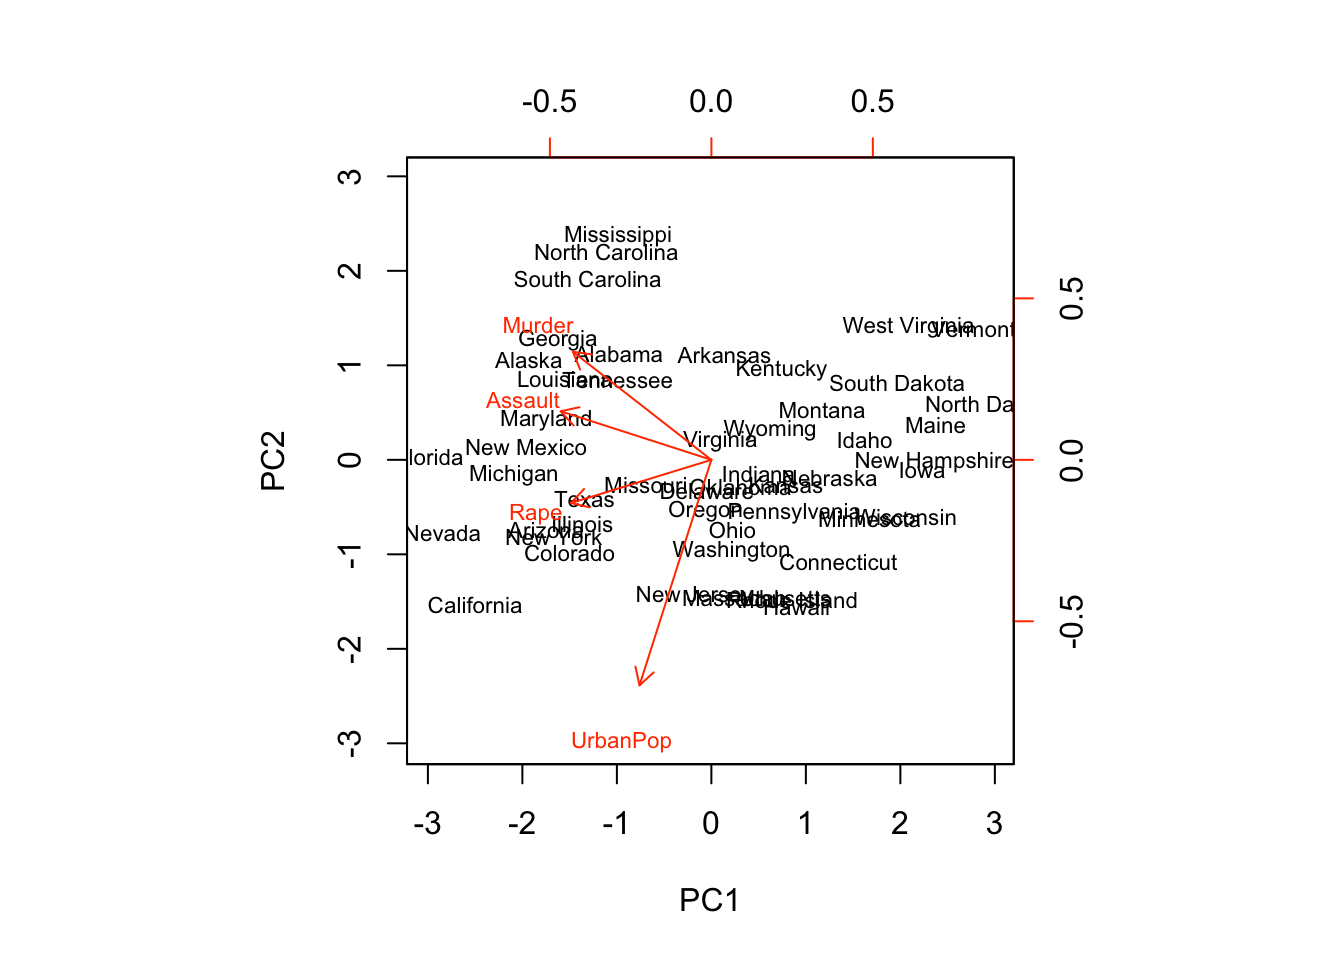
\includegraphics[width=0.7\linewidth]{USAarrests}
	\caption{\textbf{BiPlot}.
		Arrest type data for USA states. 
		Data includes urban population size, number of rape related arrests, assault related, and murder related ($p=4$). 
		Each city is presented against its two first PCs. 
		Arrows encode the loadings. 
		They show that PC1 encodes a general crime level, as it is the average of all type of crimes. 
		PC2 measures the level of urbanization, as it is dominated by the UrbanPopulation variable. 		
		\\ Source: \url{https://goo.gl/85qtKv}}
	\label{fig:usaarrests}
\end{figure}



\subsubsection{Scree Plot}
\label{sec:scree_plot}
[TODO]



\subsection{Mathematics of PCA}
\label{sec:pca_mathematics}
We now present the derivation of PCA from the two different motivations.

\subsubsection{Variance Maximizing View of PCA}

\begin{proof}
	The sketch of the proof is the following:
	We will first show that the weight vector that maximizes the variance is the eigenvector that corresponds to the first principal component.
	We will do so for the \emph{population} covariance, $\Sigma$, and wrap up by plugging its empirical counterpart, $X'X$ (assuming a centered $X$). 
		
	Starting with the first principal component.
	For a random $p$-vector, $\x$ denote $\Sigma:=\cov{\x}$, so that for a fixed $p$-vector $v$: $\cov{v'\x}=v' \Sigma v$.
	Finding a linear combination of $\x$ that best separates individuals, means maximizing $\cov{v'x}$
	w.r.t. to $v$.
	Clearly, $\cov{v'x}$ may explode if any $v$ is allowed. 
	It is most convenient, mathematically, to constrain the $l_2$ norm: $\normII{v}^2=1$.
	Maximizing under a constraint, using Lagrange-Multipliers: 
	\begin{align}
	\argmax{v}{v' \Sigma v - \lambda (\normII{v}^2-1)}.
	\end{align}
	Differentiating w.r.t $v$ and equating zero: 
	\begin{align}
	(\Sigma- \lambda I) v = 0
	\end{align}
	We thus see that any of the $p$ eigenvalue-eigenvector pairs of $\Sigma$ is a local extremum. 
	Which of them to pick?
	To find a \emph{global} maximum we return to the original problem, as plug our result:
	\begin{align}
	\label{eq:pca_maximal_variance}
	\argmax{v:\normII{v}^2=1}{v' \Sigma v }=\argmax{\lambda}{v' \lambda v }
	\end{align}
	so that the global maximum is obtained with the largest eigen-value $\lambda$.
	Put differently, the weight vector that returns the score that best separates individuals, is the eigenvector of $\Sigma$ with the largest eigenvalue. 
	
	The second principal component can be found by solving the same problem, with the additional constraint of $v_2$ orthogonal to $v_1$.
	
	The last missing ingredient is that instead of the true covariance between the features, $\Sigma$, we use the (centered) empirical covariance $X'X$.
\end{proof}


\begin{remark}
Readers familiar with matrix norms will recognize that the above is exactly the derivation of the spectral norm of $\Sigma$.
\end{remark}



\subsubsection{Linear-Space approximation view}

In here, we try to find a series of $\manifold_q; q=1,\dots,p$, such that $\manifold_q$ is a \emph{linear} subspace of dimension $q$ which well approximates $X$ in some (matrix) norm. 
For the deatils, see for instance \cite{shalev2014understanding}.




\subsubsection{Why did Hotelling and Pearson arrive to the same solution?}
\label{sec:pca_intuition}

We have currently offered two motivations for PCA: 
(i) Find linear combinations $v_1,\dots,v_p$ that best distinguish between observations, i.e., maximize variance. 
(ii) Find the linear subspaces $\manifold_1,\dots,\manifold_p$ that best approximates the data.
The reason these two problems are equivalent, is due to the use of the squares-error/Euclidean norms.

Informally speaking, the data has some total variance. 
In analogy to the $SST=SSR+SSE$ decomposition in linear regression, the total variance of $X$ can be decomposed into the part in $\manifold_q$, and the part orthogonal. 
The orthogonal part is the distance of $X$ from $\manifold_q$. 
Maximizing the variance in $\manifold_q$ is thus the same as minimizing the distance from $X$ to $\manifold_q$. 

The only unresolved matter- is why the solution to the variance maximization problem is a \emph{linear} subspace?
This is simply because all the scores, are linear combinations of columns of $X$, thus span a linear subspace, as is sought in the linear-subspace approximation view. 


\subsection{How many PCs can you recover?}
On the face of it, with $p$ variables you can find $p$ PCs. 
Things are not that simple however.

In the population version of the problem, i.e., when $\Sigma$ is known, there may be as many non zero eigenvalues as the rank of $\Sigma$. 
Stating that $\Sigma$ is full rank, is stating that the variables of $\x$ are not fully correlated.

In the empirical version of the problem, i.e., when $X'X$ is known, there may be as many non zero eigenvalues as the rank of $X'X$.
Clearly, if $p>n$, variables of $X$ have to be linearly dependent, so that $X'X$ cannot possibly be of full rank.
To say that the kernel of $X$ is of rank $p-n>0$, is to say that there are $p-n$ scores that are identically zero, thus have no variance. 


Problems do not end when $p<n$. 
This is because if $p<n$ but $p\sim n$ then we do not have many observations per estimated parameter. 
In the statistical literature, this is known as a \emph{high dimensional} problem. 
In the engineering parlance, we say we have low \emph{signal to noise}.
For a rigorous treatment of the statistical properties of PCA, see \cite{nadler2008finite}.
 





\subsection{PCA as a Graph Method}
\label{sec:pca_as_graph}

It turns out that we may find the sequence of best approximating linear subspaces, i.e., the PCs, without the actual measurements $X$, but only with a dissimilarity graph. 
In particular, with the $n\times n$ graph $\dissimilaritys$ of Euclidean distances between individuals: $\dissimilaritys_{i,j}:= \normII{x_i-x_j}$. 

It should come of no surprise that we done need the actual measurements, $X$, since the optimal loadings, $v$, only depend on the covariance $\Sigma$, or its empirical counterpart, $X'X$. 
It may, however, be quite surprising that given the distances between individuals, we may not recover the covariance between variables, $X'X$, but we can recover the PCs. 
Put differently, to find the low dimensional $\manifold$ that approximates the data, we don't need the whole data, but rather, only the graph of distances between data points. 

For proof of the above statement, we refer the reader to \cite[Sec.18.5.2]{friedman2001elements}

This observation will later be very useful for other dimensionality reduction algorithms, which operate not on the original data points, but rather, on dissimilarity graphs. 





\section{Preliminaries}

\subsection{Terminology}

\begin{tcolorbox}
	\begin{description}
		
		\item[Variable] \Aka \emph{dimension}, or \emph{feature} in the machine learning literature, or \emph{column} for reasons that will be obvious in the next item. 
		
		\item[Data] \Aka \emph{sample}, \emph{observations}, depending on your community. 
		Will typically consist of $n$, $p$ dimensional vectors, i.e., with $p$ variables in each.
		We typically denote the data as a $n\times p$ matrix $X$. 
		
		\item[Manifold] A space which is regular enough so that it is \emph{locally} has all the properties of a linear space. 
		We will denote an arbitrary manifold by $\manifold$.
		
		
		\item[Embedding] Informally speaking: a ``shape preserving'' mapping of a space into another. 
		
		\item[Linear Embedding] An embedding done via a linear operation (thus representable by a matrix). 
		
		\item[Generative Model] Known to statisticians as the \emph{sampling distribution}. 
		The assumed stochastic process that generated the observed data. 
		
	\end{description}
\end{tcolorbox}




\subsection{Motivations}

\begin{description}
	\item [Scoring] Give each observation a score (Hotelling motivation).

	\item [Latent structure] Recover unobservables from indirect measurements. 
	E.g: Blind signal reconstruction, CT scan, cryo-electron microscopy, etc. 
	
	\item [SNR] Denoise measurements before further processing like clustering, supervised learning, etc. 
	
	\item [Compression] Save on RAM ,CPU, and communication when operating on a lower dimensional representation of the data. 
	
\end{description}







\subsection{Properties of a dimensionality reduction approach}
Here are some major dimensions that characterizes dimensionality reduction approaches. 
We will try to state the characteristics of each approach as we proceed, but we are nowhere near exhaustive.
The reader is thus advised to try and place each approach along the following dimensions:
\begin{description}
	\item [Generative vs. algorithmic] Refers to the motivation of the approach. Is it stated as an algorithm, or stated via some generative probabilistic model. 
	PCA is purely algorithmic. 

	\item [Linear $\manifold$ vs. non-linear $\manifold$]. 
	Is the target manifold linear or not?
	In PCA, $\manifold$ is linear.

	\item [Linear embedding vs. non-linear embedding]. 
	Is the embedding into $\manifold$ a linear operation?
	In PCA, the embedding is linear, and indeed, represented by a matrix. 
	
	\item [Learning an embedding vs. an embedding function?]
	Will we need to apply the reduction to new data? 
	If yes, we need to learn an \emph{embedding function}. 
	If no, and we merely want to low dimensional representation of existing data, we only need to learn an embedding. 
	
	\item [Euclidean vs. non-Euclidean] 
	Many dimensionality reduction methods only need a dissimilarity (i.e. distance) graph to operate. 
	The Euclidean norm is historically the most popular.
	Some methods are agnostic to the norm used, while some, some have Euclid hard-wired into them, and some, hard-wire themselves with some other norm. 
	
\end{description}





\section{Latent Variable Generative Approaches}
All generative approaches to dimensionality reduction will specify some unobserved set of variables, which we can observe indirectly up to some measurement noise. 
The unobservable variables will typically have a lower dimension than the observables, thus, dimension is reduced. 
We start with the simplest case of linear Factor Analysis. 


\subsection{Factor Analysis (FA)}

To fix ideas, we start by revisiting the IQ problem in Example~\ref{ex:iq}:
\begin{example}[g-factor\footnote{\url{https://en.wikipedia.org/wiki/G_factor_(psychometrics)}}]
	
	Assume $n$ respondents answer $p$ quantitative questions: $x_i \in \reals^p, i=1,\dots,n$. 
	Also assume, their responses are some linear function $\loadings \in \reals^p$ of a single personality attribute, $s_i$. 
	We can think of $s_i$ as the subject's ``intelligence''.
	We thus have 
	\begin{align}
	x_i = A s_i + \varepsilon_i
	\end{align}
	And in matrix notation:
	\begin{align}
	\label{eq:factor}
	X = A \latent +\varepsilon
	\end{align}
	The problem is to recover the unobservable intelligence scores, $s_1,\dots,s_n$, from the observed answers $X$.	
\end{example}


Assuming a generative distribution on $\latent$ and $\varepsilon$, we may try to estimate $\loadings \latent$ by assuming some distribution on $\latent$ and $\varepsilon$ and apply maximum likelihood.
Under standard assumptions on the distribution of $\latent$ and $\varepsilon$, recovering  $\latent$ from $\estim{\loadings\latent}$ is still impossible as there are infinitely many such solutions.
To see this, consider an orthogonal \emph{rotation} matrix $\rotation$ ($\rotation' \rotation=I$). For each such $\rotation$: $ \loadings \latent=\loadings \rotation' \rotation \latent = \loadings^* \latent^*$.
While mathematically equivalent, $\loadings$ and $\loadings^*$ may have very different interpretations. 
This is why many researchers find FA an unsatisfactory inference tool.


\begin{remark}[Identifiability in PCA]
	The non-uniqueness (non-identifiability) of the FA solution under variable rotation is never mentioned in the PCA context. Why is this?
	This is because the methods solve different problems. 
	The reason the solution to PCA is well defined is that PCA does not seek a single $\latent$ but rather a \emph{sequence} of $\latent$ with dimensions growing from $1$ to $n$. 
\end{remark}

\begin{remark}[Linear and non-linear embeddings]
	In classical FA in Eq.(\ref{eq:factor}) is clearly an embedding to a linear space. 
	The one spanned by $\latent$. 
	Under the classical probabilistic assumptions on $\latent$ and $\varepsilon$ the embedding itself is also linear, and is sometimes solved with PCA. 
	Being a generative model, there is no restriction for the embedding to be linear, and there certainly exists sets of assumptions for which the FA embedding is non linear. 
\end{remark}

\paragraph{FA Terminology}
The FA terminology is slightly different than PCA:
\begin{itemize}
	\item \textbf{Factors}: The unobserved attributes $\latent$. 
	Not to be confused with the \emph{principal components} in the context of PCA.
	\item \textbf{Loadings}: 
	The $\loadings$ matrix; the contribution of each attribute to the observed $X$.
	\item \textbf{Rotation}: An arbitrary orthogonal re-combination of the latent attributes $\latent$ and loadings, which changes the interpretation of the result.
\end{itemize}


The FA literature does offer several heuristics to ``fix'' the solution of the FA. 
These are known as \emph{rotations}:
\begin{itemize}
	\item \textbf{Varimax}: 
	By far the most popular rotation. Attempts to construct factors that are similar to the original variables, thus facilitating interpretation. 
	This can be seen as a "soft" approach to sPCA (Sec.\ref{sec:sPCA}).
	
	\item \textbf{Quartimax}: 
	Seeks a minimal number of factors to explain each variable. 
	May thus result factors that are uninterpretable, since they all rely on the same variables.
	
	\item \textbf{Equimax}: A compromise between Varimax and Quartimax. 
	
	\item \textbf{Oblimin}: 
	Relaxes the requirement of the factors to be uncorrelated, so that they may be similar to the original variables; even more so than in varimax. 
	This facilitates the interpretability of the factors. 
	
	\item \textbf{Promax}: 
	A computationally efficient approximation of oblimin.
\end{itemize}

\subsubsection{Bibliographic Notes}
For a brief review of Factor Analysis see \cite{friedman2001elements}.
For an full exposition, and a discussion of the differences with PCA, see \cite{jolliffe2002principal}.


\subsection{Non Linear Factor Analysis}
Classical FA deals with features, $X$, that are linear in the latent factors, $\latent$. 
Like any other generative model approach, it can be easily extended to deal with non-linear functions of the latent factors: $X=g(S)$, provided that $g(.)$ is one-to-one. 
This problem is a non-linear embedding into a linear space (the one spanned by $\latent$).





\subsection{Independent Component Analysis (ICA)}
\label{sec:ica}


ICA is a family of latent space models, thus, a \emph{meta-method}.
It assumes data is generated as some function of the latent variables $\latent$. 
In many cases this function is assumed to be linear in $\latent$ so that ICA is compared, if not confused, with PCA and even more so with FA. 
In its most popular form, $X$ is assume to be a \emph{linear} function of the latent independent components: $X=\loadings \latent$.

The fundamental idea of ICA is that $\latent$ has a joint distribution of \emph{non-Gaussian independent} variables. 
This independence assumption, solves the the non-uniquness of $\latent$ in FA.

Being a generative model, estimation of $\latent$ can then be done using maximum likelihood, or other estimation principles. 
A popular information theoretic estimation principle, replacing the maximum-likelihood principle, is known as \emph{infomax}.

ICA is a popular technique in signal processing, where $\latent$ is actually the signal, such as sound in Example~\ref{ex:blind-signal}.
Recovering $\latent$ is thus recovering the original signals mixing in the recorded $X$. 



\begin{remark}[ICA and FA]
	The solutions to the (linear) ICA problem can ultimately be seen as a solution to the FA problem with a particular rotation $\rotation$ implied by the probabilistic assumptions on $\latent$.
	Put differently, the formulation of the (linear) ICA problem, implies a unique rotation, which can be thought of as the rotation that returns components that are as far from Gaussian as possible. 
\end{remark}


\begin{remark}[Linear and non-linear embeddings]
	In classical FA in Eq.(\ref{eq:factor}) is clearly an embedding to a linear space. 
	The one spanned by $\latent$. 
	Under the classical probabilistic assumptions on $\latent$ and $\varepsilon$ the embedding itself is also linear, and is sometimes solved with PCA. 
	Being a generative model, there is no restriction for the embedding to be linear, and there certainly exists sets of assumptions for which the FA embedding is non linear. 
\end{remark}


\begin{remark}[Linear and non-linear embeddings]
	In classical ICA in Eq.(\ref{eq:factor}) is clearly an embedding to a linear space. 
	The one spanned by $\latent$. 
	The probabilistic assumptions on $\latent$ and $\varepsilon$ the embedding itself being non linear, thus solved as an optimization problem, and not via PCA. 
\end{remark}




\subsubsection{Mathematics of ICA}
For ease of presentation we present a simple setup, which can be considerably generalized. 
In this setup, we will first analyze the population problem, i.e., in terms of random variables. 
We thus replace the data $X$, with the random vector $\x$, and afterwards consider implementation for finite samples. 
\begin{itemize}
	\item $\x=\loadings \latent$, implying that $\x$ is \emph{linear} in the latent components, and the latent space is of dimension $\rank=p$. It follows that $s=\loadings'X$.
	\item $\x$ has been pre-whitented, so that $\cov{\x}=I$.
	\item Distance between distributions are measured using the Kullback-Leibler divergence (KL): $\kl{\x}{\latent}$.
\end{itemize}

The optimization problem in this simple ICA is to find an orthogonal matrix $\loadings$, for which:
(i) the components of $\loadings'\x$ are independent;
(ii) $\loadings'\x$ is a good approximation of $\x$.
Formally: 
\begin{align}
\label{eq:ica_optimization}
\argmin{\loadings \text{ orthogonal} \;; \loadings'\x \text{ independent}}{\kl{\loadings'\x}{\x}}.
\end{align}


By enforcing the independence constraint in Eq.(\ref{eq:ica_optimization}), and due to the properties of the KL divergence, Eq.(\ref{eq:ica_optimization}) is equivalent to
\begin{align}
\label{eq:ica_optimization2}
\argmin{\loadings \text{ orthogonal}}{\sum_{j=1}^{\rank} \entropy(\loadings_j\x)- \entropy(\x)}
\end{align}
where $\entropy(\x)$ denotes the Entropy of the random variable $\x$ (Definition \ref{def:entropy}).
Now, $\entropy(\x)$ is obviously fixed, so we need to minimize $\entropy(\loadings_j\x)$. 
A classical result in information theory, is that the Gaussian distribution has the maximal entropy. 
Minimizing $\entropy(\loadings_j\x)$ can thus be interpreted as finding a matrix $\loadings$ such that its columns return random variables, $\loadings_j\x$, that are as \emph{non-Gaussian} as possible.

This is where the population analysis ends. 
The insight we take from it, is that finding independent components, is actually finding non-Gaussian combinations of $\x$. 
The different implementations of ICA, indeed look for a matrix $\loadings$ which returns the most non-Gaussian combinations of the observed $X$. 








\subsubsection{Bibliographic notes}
For a general discussion of ICA see \cite{jolliffe2002principal}.
For a brief exposition of the linear ICA see \cite{friedman2001elements}. 
For a detailed review of ICA see \cite{hyvarinen2000independent}. 








\section{Purely Algorithmic Approaches}

We now discuss dimensionality reduction approaches that are not stated via their generative model, but rather, directly as an algorithm.
This does not mean that they cannot be cast via their generative model, but rather they were not motivated as such.



\subsection{Multidimensional Scaling (MDS)}
\label{sec:mds}

Very roughly speaking, MDS can be thought of as a variation on PCA, that begins with a distance graph\footnote{The term Graph is typically used in this context instead of Network. But a graph allows only yes/no relations, while a network, which is a weighted graph, allows a continuous measure of similarity (or dissimilarity). It is thus more appropriate.} $\dissimilaritys$, and embeds into a two-dimensional space.
We have already seen in Section~\ref{sec:pca_as_graph} that PCA really only needs a similarity graph. 
The embedding into two dimensions is motivated by that fact that MDS is typically used for visualization. 

MDS aims at embedding a graph of distances, while preserving the original distances.
Basic results in graph/network theory suggest that the geometry of a graph cannot be preserved when embedding it into lower dimensions. 
The differences between MDS algorithms thus rests in the penalization for geometric distortions. 

\begin{remark}[MDS and PCA]
	If the input of MDS is the Euclidean distances between points, then MDS with ``classical scaling'' (\aka Torgerson scaling) returns the exact same embedding as PCA with $2$ PCs.
\end{remark}


The embedding is merely the assigning of each point to a location in some lower dimensional linear space $\manifold$. 
The assignment is driven by a \emph{stress function} which penalizes for the average distortion created by the embedding.
The different types of MDSs, such as \emph{Classical MDS}, and \emph{Sammon Mappings}, differ in the stress function driving the embedding.

Sadly, MDS may scale poorly to large dissimilarity matrices, and the optimization may converge to a local minimum.
Being a data embedding, and not an embedding function, when new data points are made available, the embedding will have to be re-learned.

For more on MDS see Section 14.8 in \cite{hastie_elements_2003} or \cite{borg_modern_2005}.



\subsubsection{Non-Metric MDS}
[TODO]


\paragraph{Mathematics of MDS}
We start with either a dissimilarity network $\dissimilaritys=(\dissimilarity_{i,j})$, or a similarity network $\similaritys=(\similarity_{i,j})$.
Similarities can be thought of as correlations, and dissimilarities as distances (which are indeed the typical measures in use).
Define $z_i \in \reals^\rank$ the location of point $i$ in the target linear space of rank $\rank$. 
The $z_i$'s are set to minimize some penalty for geometric deformation called the \emph{stress function}.
Typical stress functions include:
\begin{description}
	
	\item[Classical MDS] Using the centred inner product (i.e. empirical covariance) as the similarity measure and minimizes the squared distortion:
	$\similarity_{i,j}:= \scalar{x_i-\bar x}{x_j-\bar{x}}$ and the new location are given by
	\begin{align}
	\label{eq:mds_classical}
	\argmin{z_1,\dots,z_n}{\sum_{i,j=1}^{n} (\similarity_{i,j}-\scalar{z_i-\bar z}{z_j-\bar{z}} )^2}.
	\end{align}
	
	\item[Least Squares] Also known as \emph{Kruskal-Shepard}. Also minimizes the squared distortion. 
	\begin{align}
	\label{eq:mds_stress}
	\argmin{z_1,\dots,z_n}{\sum_{i \neq j} (\dissimilarity_{i,j}-\norm{z_i-z_j} )^2}.
	\end{align}
	
	\item[Sammon Mapping] Also known as \emph{Sammon's stress}, aims at minimizing the \emph{proportion} of distortion:
	\begin{align}
	\label{eq:mds_sammon}
	\argmin{z_1,\dots,z_n}{\sum_{i \neq j} \frac{(\dissimilarity_{i,j}-\norm{z_i-z_j} )^2}{\dissimilarity_{i,j}}}.
	\end{align}
	
\end{description}


\begin{remark}[Classical and Least Squares MDS]
	Although they both minimize the squared distortion, working with $\similaritys$ or $\dissimilaritys$ lead to different solutions. 
	In particular, Classical is a linear embedding while Stress is not. 
\end{remark}





\subsection{Force Embedding}




\subsection{Local MDS}
\label{sec:localMDS}
Local MDS is motivated by the observation that if the data does not lay in a globally convex subspace, then global distances are a very distorted measure, whereas geodesic distances should be used instead. 
Their solution is to compute $\dissimilaritys$ using only local distances, and then calling upon MDS.

\begin{remark}[The Non-Linearity of Local MDS]
	\label{remark:linearity_of_localMDS}
	Local MDS is typically considered a non-linear-space embedding, thus belonging to Section \ref{sec:dim_reduce_nonlinear}.
	I currently do not think is the case, as it is presented as a linear space embedding.
	Maybe Remark \ref{remark:nldr} can explain the confusion in terminology.
\end{remark}






\subsection{Isometric Feature Mapping (Isomap)}
\label{sec:isomap}

Isomap, also known as \emph{principal coordinate analysis}, is another method intimately related to MDS(\S\ref{sec:mds}).\marginnote{Principal Coordinate Analysis}

Isomap follows the same motivation as Local MDS (\S\ref{sec:localMDS}), but with a different algorithm to compute the dissimilarity matrix $\dissimilaritys$.

\begin{remark}[The Non-Linearity of Isomap]
	Just like Local MDS, Isomap is typically considered a non-linear-space embedding (see Remark \ref{remark:linearity_of_localMDS}).
	I currently do not think is the case.
\end{remark}









% % % % Non linear dimensionality reduction % % % % %
\section{Non-Linear-Space Embeddings}
\label{sec:dim_reduce_nonlinear}

We now 



Section \ref{sec:dim_reduce_linear} deals with representing the data in a \emph{linear} sub space $\manifold$. They all aim at finding a basis which efficiently represents that data, with respect to some target function. 
In this section, we allow $\manifold$ to be non-linear. 
We will thus no longer be able to represent the data by its coordinates in some basis.


\begin{remark}[Non Linear Dimensionality Reduction]
	\label{remark:nldr}
	Do not let the title of this section be confused with the term Non-Linear Dimensionality-Reduction (NLDR).
	NLDR deals with the nature of the \emph{embedding} operation, and not with the structure of the target manifold $\manifold$ (see also Remark \ref{remark:linear}).\marginnote{NLDR}
	This section deals with embeddings into a non-linear subspace, regardless of the nature of the embedding operator.
	Cases of non-linear embeddings (NLDR) into a \emph{linear} manifolds $\manifold$ belong in Section~\ref{sec:dim_reduce_linear}.
\end{remark}




\subsection{Kernel Principal Component Analysis (kPCA)}
\label{sec:kpca}

Back to the motivating example from the PCA section (\S\ref{sec:pca}): assume we want to construct a ``bigness'' score, that best separates between individuals, but we no longer constrain it to be a linear function of the height and weight.
Recalling that the best discrimination between observations means maximizing the variance of the \emph{scores} given to individuals, we could try to find the best separating score $g(x)$ by solving 
\begin{align}
\label{eq:kpca_wrong}
\argmax{g}{\covn{g(X)}}
\end{align}
where $g(x)$ maps an individual's features to a score in $\manifold$.

Alas, just like in the supervised learning problem, without any constraints on $\manifold$, thus on $g$, we might overfit \andor not be able to compute $g$ as optimization is done in a infinite dimensional space. 
We thus have two matters to attend:
(i) We need to constrain $g(x)$ so that it does not overfit.
(ii) We need the problem to be computable.
This is precisely the goal of kPCA. 

We have already encountered a similar problem with Smoothing Splines (\S\ref{sec:smoothing_splines}). It is thus not surprising that the solution has the same form. 
Namely, if we choose the right $g$'s, the solution of Eq.(\ref{eq:kpca_wrong}) takes a very simple form. 
The classes of such $g$'s are known as Reproducing Kernel Hilbert Spaces (RKHS). 
They are discussed in Appendix~\ref{apx:rkhs}.



\paragraph{Mathematics of kPCA}
[TODO]




\subsection{Self Organizing Maps (SOM)}
SOMs, are a non-linear-subspace dimensionality reduction method, aimed at good clustering. 
It is non-linear because the algorithm (which cannot be cast as an ERM problem) returns an embedding into a non-linear manifold.
More details in Section~\ref{sec:som}.



\subsection{Principal Curves and Surfaces}


Principal curves (or surfaces), is an algorithm. It cannot be cast as an optimization problem.
Being a non-linear space embedding method, the algorithm iterates until it returns a curve of a surface.
In the curve case, it will return a curve with the \emph{self consistency} property. I.e., a curve with a path that is the average of all it's closest data points.\marginnote{Self Consisntecy}
Roughly speaking, one can think of this curve as a parametrized function, connecting all the k-means cluster centres in the smoothest way possible.
Using the same, slightly inaccurate depiction, a principal surface is a \emph{surface} connecting these k-means cluster centres.
We stress that in both cases, the output is a continuous parametrization of the curve or the surface.

It is highly uncommon to approximate the data with surfaces (manifolds) with a dimension larger than $2$, as typically the method is used for projecting the data before visualizing \andor clustering.






\subsection{Local Linear Embedding (LLE)}
\label{sec:lle}



LLE aims at finding linear subspaces that are good approximations of small neighbourhoods of the whole data $X$.
It is similar in spirit to Isomap (\S\ref{sec:isomap}) and LocalMDS (\S\ref{sec:localMDS}).
It differs, however, in the way similarities are computed, and in the way embeddings are performed. 
In particular, as the name may suggest, LLE performs local embeddings to linear subspaces. The resulting approximating manifold $\manifold$, being the ``stitching'' of many linear spaces, is ultimately non linear.




\subsection{Auto Encoders}
\label{sec:auto_encoders}
[TODO. AKA auto-associator or Diabolo network]



\subsection{Matrix Factorization}
\label{sec:matrix_factorization}
[TODO- is it generative?]



\subsection{Information Bottleneck}
[TODO]

%The \emph{information bottleneck} is an information theoretic framework, due to \cite{tishby_information_1999}, that generalizes the idea of dimensionality reduction and data compression.
%It is a general statement of the problem of maximal compression of $X$, while preserving as much of the information in $X$ as possible.
%To state the general problem we require some definitions from information theory.
%
%\begin{definition}[Entropy]
%The entropy of a random variable $\x$ is defined as the expected negative log density of $\x$: 
%$$\expect{-\log \pdf(\x)}.$$
%\end{definition}
%
%\begin{definition}[Mutual Information]
%The mutual information between two random variable $\x$ and $\y$ is defined as : 
%$$\expect{\log \frac{\pdf(\x,\y)}{\pdf(\x) \pdf(\y)}}.$$
%\end{definition}
%
%Informally speaking, the entropy is a measure of the variability of a distribution, and the mutual information is a measure of deviation from independence, i.e., captures the amount of information $\x$ carries on $\y$, and vice-versa.
%With this intuition, and denoting the compression of $x$ by $y=g(x)$, we may define the compression problem as:
%\begin{align}
%	\argmin{g}{arg2}
%\end{align}


\begin{remark}[Information Bottleneck and ICA]
	[TODO]
\end{remark}











\section{Dealing with the high-dimension}

\subsection{Sparse Principal Component Analysis}
\label{sec:sPCA}




\newpage
\bibliographystyle{abbrvnat}
\bibliography{dim_reduce.bib}



\end{document}
